% SC1008 — Chapter 3: Arrays, Strings, Structs (0->100 ground-up)
\chapter{Arrays, Strings, and Structs: Building Bigger Boxes}
\label{ch:arrays-strings-structs}

\begin{quote}
\emph{``Bad programmers worry about the code. Good programmers worry about data structures.''} --- Linus Torvalds. We now aggregate bytes into arrays, text into strings, and records into structs.
\end{quote}

\noindent\fbox{\parbox{\dimexpr\linewidth-2\fboxsep-2\fboxrule}{%
\textbf{From zero: arrays are just many boxes in a row.} We start with contiguous storage, show why indexing is arithmetic, then build strings (char arrays + terminator) and structs (heterogeneous boxes) with pictures before code.}}

\section*{Learning Outcomes}
After this chapter you will be able to:
\begin{enumerate}[label=(L\arabic*)]
    \item declare, initialise, and index arrays and explain bounds checking (or lack thereof);
    \item manipulate C strings safely with \texttt{<string.h>} functions;
    \item define and use \texttt{struct} types with correct member access;
    \item relate arrays to pointers and explain decay and \texttt{sizeof} pitfalls;
    \item design a small record type and its helper functions.
\end{enumerate}

% ============================================================
\section{Arrays: Contiguous Homogeneous Storage}
\label{sec:arrays}
An array packs \texttt{N} elements of the same type contiguously. The name \texttt{a} is the address of element 0; \texttt{a[i]} means \texttt{*(a+i)}.

\begin{figure}[h]\centering
\begin{tikzpicture}[scale=0.70,every node/.style={font=\scriptsize}]
\foreach \i/\v in {0/11,1/22,2/33,3/44,4/55} {
  \pgfmathsetmacro{\x}{\i*1.65}
  \draw[thick,fill=blue!12] (\x,0) rectangle (\x+1.45,0.85);
  \node at (\x+0.72,0.48) {\texttt{\v}};
  \node[font=\tiny,fill=white,inner sep=1pt] at (\x+0.72,0.15) {\texttt{[\i]}};
  \node[font=\tiny] at (\x+0.72,-0.28) {\tiny\texttt{+0x\i*4}};
}
\node[font=\tiny,fill=orange!15,rounded corners=2pt,inner sep=2pt] at (1.2,1.30) {\texttt{int a[5]}};
\draw[-{Latex},thick,red!70!black] (0.72,-0.55)--(0.72,-0.05);
\node[font=\tiny,red!70!black] at (0.72,-0.80) {\texttt{a}};
\node[font=\tiny,fill=yellow!12,rounded corners=2pt,inner sep=2pt] at (5.5,1.30) {\texttt{a[2] $\equiv$ *(a+2)}};
% bounds illustration
\draw[thick,red!60!black,dashed] (8.25,0) rectangle (9.70,0.85);
\node[font=\tiny,red!60!black] at (8.97,0.42) {out of bounds};
\node[font=\tiny,red!60!black] at (8.97,-0.28) {UB!};
\end{tikzpicture}
\caption{Array layout: 5 contiguous \texttt{int}s. Indexing is pointer arithmetic. Accessing beyond \texttt{[4]} is undefined behaviour (no bounds check in C).}
\label{fig:array-layout}
\end{figure}

\begin{lstlisting}[language=C]
int a[5] = {11,22,33,44,55};  // initialise
int b[5] = {0};               // all zero
// int c[5] = {1,2};          // remainder zero-filled
for(int i=0;i<5;i++) printf("%d ", a[i]);
printf("\nsize=%zu bytes\n", sizeof(a)); // 20 = 5*4
// void f(int x[5]) -- inside f, sizeof(x) == sizeof(int*) !
\end{lstlisting}
C does \emph{no} bounds checking. \texttt{a[5]} or \texttt{a[-1]} compiles but reads/writes arbitrary memory --- a classic security hole. Multi-dimensional arrays are arrays of arrays: \texttt{int m[2][3]} is 6 ints row-major.

\section{C Strings: Char Arrays with a Sentinel}
\label{sec:strings}
A C string is a \texttt{char} array terminated by \texttt{'\textbackslash0'} (value 0). The terminator marks the end; the array length may be larger.

\begin{figure}[h]\centering
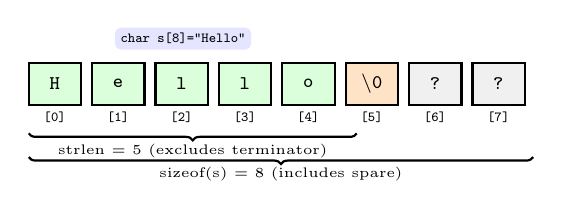
\begin{tikzpicture}[scale=0.70,every node/.style={font=\scriptsize}]
\foreach \i/\ch in {0/H,1/e,2/l,3/l,4/o,5/\textbackslash0,6/?,7/?} {
  \pgfmathsetmacro{\x}{\i*1.15}
  \ifnum\i<6 \def\col{green!14}\else\def\col{gray!12}\fi
  \ifnum\i=5 \def\col{orange!22}\fi
  \draw[thick,fill=\col] (\x,0) rectangle (\x+0.95,0.75);
  \node at (\x+0.47,0.38) {\texttt{\ch}};
  \node[font=\tiny] at (\x+0.47,-0.22) {\texttt{[\i]}};
}
\node[font=\tiny,fill=blue!10,rounded corners=2pt,inner sep=2pt] at (2.8,1.20) {\texttt{char s[8]="Hello"}};
\draw[decorate,decoration={brace,mirror},thick] (0,-0.52)--(5.95,-0.52) node[midway,below,font=\tiny] {strlen = 5 (excludes terminator)};
\draw[decorate,decoration={brace,mirror},thick] (0,-0.95)--(9.15,-0.95) node[midway,below,font=\tiny] {sizeof(s) = 8 (includes spare)};
\end{tikzpicture}
\caption{A C string \texttt{"Hello"} in an 8-byte buffer. \texttt{strlen} counts to \texttt{\textbackslash0}; \texttt{sizeof} counts the whole array.}
\label{fig:cstring}
\end{figure}

\begin{lstlisting}[language=C]
#include <string.h>
char s[16] = "Hello";          // 6 bytes used, 10 spare
printf("%zu %zu\n", strlen(s), sizeof(s)); // 5 16
strcpy(s, "Hi");               // copies including \0
strcat(s, "!");                // appends: "Hi!"
// DANGER: strcpy with no bounds check -- use strncpy/strlcpy or snprintf
snprintf(s, sizeof(s), "%s", "Hello, NTU!"); // safe, always terminates
for(int i=0; s[i]!='\0'; i++) putchar(s[i]);
\end{lstlisting}
String literals like \texttt{"Hi"} live in read-only memory; writing to them is UB. Always ensure a \texttt{\textbackslash0} and enough space.

\section{Structs: Heterogeneous Records}
\label{sec:structs}
A \texttt{struct} groups different types into one compound type. Each \emph{member} has its own offset.

\begin{figure}[h]\centering
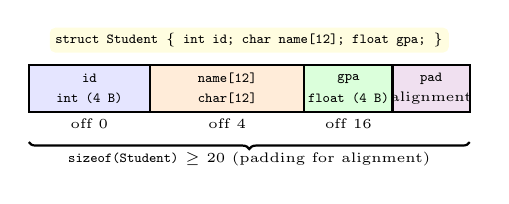
\begin{tikzpicture}[scale=0.70,every node/.style={font=\scriptsize}]
\draw[thick,fill=blue!10] (0,0) rectangle (2.2,0.85);
\node[font=\tiny\bfseries] at (1.1,0.60) {\texttt{id}};
\node[font=\tiny] at (1.1,0.25) {\texttt{int (4 B)}};
\draw[thick,fill=orange!15] (2.2,0) rectangle (5.0,0.85);
\node[font=\tiny\bfseries] at (3.6,0.60) {\texttt{name[12]}};
\node[font=\tiny] at (3.6,0.25) {\texttt{char[12]}};
\draw[thick,fill=green!14] (5.0,0) rectangle (6.6,0.85);
\node[font=\tiny\bfseries] at (5.8,0.60) {\texttt{gpa}};
\node[font=\tiny] at (5.8,0.25) {\texttt{float (4 B)}};
\draw[thick,fill=violet!12] (6.6,0) rectangle (8.0,0.85);
\node[font=\tiny\bfseries] at (7.3,0.60) {\texttt{pad}};
\node[font=\tiny] at (7.3,0.25) {\tiny alignment};
\node[font=\tiny] at (1.1,-0.22) {off 0};
\node[font=\tiny] at (3.6,-0.22) {off 4};
\node[font=\tiny] at (5.8,-0.22) {off 16};
\draw[decorate,decoration={brace,mirror},thick] (0,-0.55)--(8.0,-0.55) node[midway,below,font=\tiny] {\texttt{sizeof(Student)} $\ge$ 20 (padding for alignment)};
\node[font=\tiny,fill=yellow!12,rounded corners=2pt,inner sep=2pt] at (4.0,1.30) {\texttt{struct Student \{ int id; char name[12]; float gpa; \}}};
\end{tikzpicture}
\caption{Struct layout: members placed in order with possible padding for alignment. \texttt{sizeof} includes padding.}
\label{fig:struct-layout}
\end{figure}

\begin{lstlisting}[language=C]
struct Student{
    int   id;
    char  name[32];
    float gpa;
};
struct Student s = {123, "Asha", 4.8f};
printf("%s %.1f\n", s.name, s.gpa);
struct Student *ps = &s;
printf("%d\n", ps->id);        // -> for pointer to struct
// array of structs
struct Student cohort[50];
cohort[0].id = 1;
\end{lstlisting}
Access via \texttt{s.member} or \texttt{ps->member} (shorthand for \texttt{(*ps).member}). The compiler may insert padding between members for alignment; never assume \texttt{sizeof} equals sum of members. Use \texttt{typedef} to alias: \texttt{typedef struct Student Student;}.

\section{Arrays vs.\ Pointers --- Decay}
In most expressions, an array \emph{decays} to a pointer to its first element. Exceptions: \texttt{sizeof(a)}, \texttt{\&a}, and string literal initialisation. Hence function parameters declared as \texttt{int a[]} are really \texttt{int *a}; the callee cannot know the length --- pass it explicitly: \texttt{void print(int *a, int n)}.


\section{Searching and Sorting Arrays}
With arrays we can implement linear search and bubble sort --- the algorithmic core of SC1007, previewed here.

\begin{lstlisting}[language=C]
int linear_search(const int *a, int n, int key){
    for(int i=0;i<n;i++) if(a[i]==key) return i;
    return -1; // not found
}
void bubble_sort(int *a, int n){
    for(int i=0;i<n-1;i++)
        for(int j=0;j<n-1-i;j++)
            if(a[j]>a[j+1]){ int t=a[j]; a[j]=a[j+1]; a[j+1]=t; }
}
\end{lstlisting}
\texttt{linear\_search} is $O(n)$; \texttt{bubble\_sort} is $O(n^2)$. The sorted array can then be binary-searched in $O(\log n)$ --- a theme of Ch.~7's \texttt{std::sort}/\texttt{find}.

\section{Nested Structs and Typedef}
Structs can contain other structs, enabling hierarchical records.

\begin{lstlisting}[language=C]
struct Date{ int day, month, year; };
struct Student{
    int id;
    char name[32];
    float gpa;
    struct Date enrolled;
};
typedef struct Student Student; // alias: Student instead of struct Student
Student s = {123, "Asha", 4.8f, {15, 8, 2024}};
printf("%02d/%02d/%04d\n", s.enrolled.day, s.enrolled.month, s.enrolled.year);
Student *ps = &s;
ps->gpa = 4.9f; // -> for pointer
\end{lstlisting}
\texttt{typedef} shortens declarations; modern C++ prefers \texttt{using Student = struct Student;}. Nested access chains like \texttt{s.enrolled.year} read left to right: ``student's enrolment date's year''.


\section{Common Pitfalls and Safe String Handling}
C's string functions are notoriously unsafe. Prefer bounded variants and always ensure termination.

\begin{lstlisting}[language=C]
char dst[8];
// UNSAFE: strcpy(dst, "Hello, NTU!"); // 12 bytes into 8 -- overflow!
snprintf(dst, sizeof(dst), "%s", "Hello, NTU!"); // safe: truncates to "Hello, "
printf("dst='%s' len=%zu\n", dst, strlen(dst));   // dst='Hello, ' len=7

char a[16]="Hello", b[]=" World";
// strncat with remaining space
strncat(a, b, sizeof(a)-strlen(a)-1); // leaves room for \0
printf("%s\n", a); // Hello World

// Tokenising (destructive)
char line[]="one,two,three";
for(char *tok=strtok(line,","); tok; tok=strtok(NULL,",")) printf("[%s]\n", tok);
\end{lstlisting}
Rule: every \texttt{char} buffer has a size; every string op must respect it. When in doubt, use \texttt{snprintf} and check its return value (needed length).

\section{Chapter Notes}
C strings are a frequent source of buffer overflows; modern code prefers bounded functions (\texttt{snprintf}, \texttt{strncpy}). C++ \texttt{std::string} (Ch.~7) eliminates the terminator bookkeeping entirely.

\section{Exercises}
\begin{enumerate}[label=E3.\arabic*, leftmargin=*, itemsep=0.6em]
\item \textbf{sizeof trap.} \texttt{int a[10];} What are \texttt{sizeof(a)} and \texttt{sizeof(\&a)}? Write a function \texttt{void foo(int a[10])} and explain why \texttt{sizeof(a)} inside \texttt{foo} differs.
\item \textbf{String length.} Implement \texttt{int my\_strlen(const char *s)} without using \texttt{<string.h>}. Why must the parameter be \texttt{const char*}?
\item \textbf{Off-by-one.} This copies unsafely: \texttt{char dst[8]; strcpy(dst,"Hello, NTU!");} How many bytes are written? Fix it with \texttt{snprintf} and explain the truncation behaviour.
\item \textbf{Struct padding.} Given \texttt{struct S\{char c; int i; char d;\};} predict \texttt{sizeof(struct S)} on a 4-byte-aligned machine. Verify with \texttt{printf("\%zu", sizeof(struct S))}.
\item \textbf{Record design.} Define \texttt{struct Course\{char code[8]; int au; float grade;\}} and write \texttt{float gpa(struct Course *cs, int n)} computing the AU-weighted GPA.
\end{enumerate}
% End of Chapter 3
